%=================================================================% 
% thesis.tex																						  
%
% Updated: May 2019
%                                        
% Main file for compiler which:                                 
%	+ Defines the custom fields used in MAThesisOutputFormat.sty,
%   + Offers "final" vs "draft" formatting for speedy compiling 
%		during edits,
%   + Uses standalone package to allow the use of \input command 
%		while ignoring preambles of subfiles, 
%   + Uses BibLaTeX by default; bibtex code is in the comments, 
%   + Calls on content.tex, which contains actual content,
%   ! Uses the file thesis.bib for references,
%   ! Displays a list of tables and list of figures by default, 
%		please visit lines 279 to 281 of MAThesisOutputFormat.sty
%		to comment out the lines as necessary.
%
%=================================================================%



% Note the extra space at the end, which is unfortunately necessary:      
\newcommand\myname{Your Name }
\newcommand\mytitle{YOUR TITLE } % The graduate division requires this to be in caps.
\newcommand\mydegree{Master of Arts } % change to  Master of Science if applicable
\newcommand\myfield{Your Field } % e.g., Mathematics
\newcommand\thismonth{Month } % graduation month: May / August / December
\newcommand\thisyear{Year } % e.g., 2014
\newcommand\myadviser{Your adviser } % Adviser
\newcommand\myadviserstitle{Associate Professor }
\newcommand\committeememberone{Your committee member } % Committee member 1
\newcommand\committeememberonetitle{Assistant Professor } 
\newcommand\committeemembertwo{Your committee member } % Committee member 2
\newcommand\committeemembertwotitle{Professor }

\documentclass[12pt,oneside]{sfsuthesis}  


%==================================================================% 
%                                                                  %
%      WHEN THESIS IS COMPLETED, CHANGE THE NEXT LINE FROM         %    
%		                                                           % 
%		                  draft TO final,                          %
%                                                                  %
% to change format according to the Graduate Division's guidelines %
%                                                                  %
%==================================================================% 
\usepackage[draft]{MAThesisOutputFormat}

\RequirePackage{standalone}


%==========%
% biblatex %
%==========%

\usepackage[backend=biber,style=numeric]{biblatex}
\addbibresource{thesis.bib}



%=========================%
% CUSTOM PACKAGES GO HERE %
%=========================%
%\usepackage{TCbasic}


\begin{document}

\thesistitle

% Main body of work:
% content.tex, to be used with thesis.tex
% This contains the main work of your thesis

\documentclass{article}
\usepackage[utf8]{inputenc}

\title{     }
\author{     }
\date{     }

\usepackage{xcolor}
\begin{document}

\chapter{Introduction}

Here's where you text starts. You might (but don't have to) have sections like\dots

\section{Introduction to the Introduction}

\dots or subsections\dots

\subsection{Introduction to the Introduction to the Introduction}

To include text in your document, you just type. You don't have to worry about spacing between sentences; \LaTeX \ does that automatically. 
To start a new paragraph, just insert an empty line.

Here comes the new paragraph. You can include tables, such as Table \ref{tablename}, which can also be turned if necessary, as seen, e.g. in Table~\ref{tablenameturned}. (I
think the latter is automatically on its own page; the former will just be put where \LaTeX \ thinks it fits best.)

\begin{table}[htb]
\begin{center}
\begin{tabular}{c||r|r|r|r|r|r|r|r}
$d$ & 2 & 3 & 4 & 5 & 6 & 7 & 8 & 9 \\ 
\hline
\text{bound} & 3.6 & 8.5 & 15.8 & 25.7 & 38.3 & 53.5 & 71.4 & 92.0
\end{tabular}
\end{center}
\caption{Bounds in various dimensions $d$.}
\label{tablename}
\end{table}

\begin{sidewaystable}
\begin{center}
\begin{tabular}{c||r|r|r|r|r|r|r|r}
$d$ & 2 & 3 & 4 & 5 & 6 & 7 & 8 & 9 \\ 
\hline
\text{bound} & 3.6 & 8.5 & 15.8 & 25.7 & 38.3 & 53.5 & 71.4 & 92.0
\end{tabular}
\end{center}
\caption{More bounds in various dimensions $d$.}
\label{tablenameturned}
\end{sidewaystable}

To start a new chapter, you don't need to add a pagebreak\dots

\chapter{The Real Stuff}

\dots \LaTeX \ does that automatically.

\section{Various Tricks}

Here are a few tidbits that came to my mind, in no particular order\dots

I'm sure most people know about {\tt $\backslash$label} and {\tt $\backslash$ref}; this feature is enough reason for me to use \LaTeX. 
For example, you might have something like\dots

\begin{theorem}[Euler]\label{eulerthm}
Leonhard says $e^{ 2 \pi i } = 1$.
\end{theorem}

\dots which you can then later (or earlier) reference as Theorem \ref{eulerthm} and you can point to page \pageref{eulerthm} on which it appears.
If you label equations like
\begin{equation}\label{eulereq}
  e^{ 2 \pi i } = 1 \, ,
\end{equation}
you can reference them most lazily using \eqref{eulereq}.

\def\v{{\mathbf v}}
\def\P{{\mathcal P}}
\def\Z{\mathbb{Z}}
\newcommand\floor[1]{\left\lfloor {#1} \right\rfloor} 

There are two ways to define internal macros: {\tt $\backslash$def} and {\tt $\backslash$newcommand}. The difference is that the former overwrites any possibly existing command,
where as the latter induces a \LaTeX \ complaint if you're redefining an existing command (in which case you should use {\tt $\backslash$renewcommand} instead). Since I'm lazy,
I tend to use {\tt $\backslash$def}, with one important exception: {\tt $\backslash$newcommand} allows you to use arguments. For example, the definition
\begin{verbatim}
\newcommand\floor[1]{\left\lfloor {#1} \right\rfloor} 
\end{verbatim}
produces a flexible floor function $\floor{\frac{ 3\pi }{ 2 }}$. And yes, the {\tt [1]} can be replaced by {\tt [n]} if you have use for {\tt n} arguments (which get the
placeholders {\tt \#1}, {\tt \#2}, \dots, {\tt \#n}).

The previous example reminds me to strongly recommend the use of {\tt $\backslash$left} and {\tt $\backslash$right} whenever you use parentheses:
\[
  ( \frac a b - 2 ) \ \text{ just doesn't look good compared with } \ \left( \frac a b - 2 \right) .
\]

There are three dashes in \LaTeX---one like the one you just saw, one that's used in ``Berndt--Zaharescu's Theorem" or ``Chapter 7--9," and one that's used in ``well-known
identity."

\newcommand{\todo}[1]{\par \noindent
  \framebox{\begin{minipage}[c]{0.95 \textwidth} TO DO:
      #1 \end{minipage}}\par}

One of my favorite packages is {\tt enumerate}:
\begin{enumerate}[{\bf i)}]
  \item first item
  \item second item
  \item third item
  \item \dots
\end{enumerate}

\todo{I stole the idea of a to-do box from a friend. This is useful when editing a paper and you want to remind your co-author or yourself about something\dots}

\textcolor{
When writing text that require many sittings, I enjoy changing the font color, which is an easy way to show progress in a long project. 

\documentclass{article}
\usepackage[utf8]{inputenc}

\title{     }
\author{     }
\date{     }

\begin{document}

For writing big files, you may separate your files into subfiles. For example, this paragraph is in \texttt{subfile.tex}. I inputted this file into \texttt{content.tex} by using the "standalone" package and the following command where the sentence should be with the following command:
\begin{verbatim}
\documentclass{article}
\usepackage[utf8]{inputenc}

\title{     }
\author{     }
\date{     }

\begin{document}

For writing big files, you may separate your files into subfiles. For example, this paragraph is in \texttt{subfile.tex}. I inputted this file into \texttt{content.tex} by using the "standalone" package and the following command where the sentence should be with the following command:
\begin{verbatim}
\input{subfile.tex} 
\end{verbatim} 
Naturally, subfiles can contain more subfiles.

\end{document}






% TLC 
\end{verbatim} 
Naturally, subfiles can contain more subfiles.

\end{document}






% TLC

%%%%%%%%%%%%%%%%%%%%%%%%%%%%%%%%%%%%%%%%%%%%%%%%%%%%%%%%%%%%%%%%%%%%%%%%%%%

\section{Math}

You can put a $\Box$ at the end of a math line if a proof happens to end with a math line. The version\dots

\begin{proof}
This follows from
\[
  e^{ 2 \pi i } = 1 \, .
\]
\end{proof}

\noindent
\dots wastes space and doesn't look nearly as cool as\dots

\begin{proof}
This follows from
\[
  e^{ 2 \pi i } = 1 \, . \qedhere
\]
\end{proof}

Speaking about proofs, sometimes you need a paragraph or two between a theorem and its proof, in which case you can use\dots

\begin{proof}[Proof of Theorem \ref{eulerthm}]
This follows from
\[
  e^{ 2 \pi i } = 1 \, . \qedhere
\]
\end{proof}

\def\lcm{\operatorname{lcm}}

You can (and should) define your own math operators with {\tt $\backslash$operatorname}. For example,
\[
  \lcm (2, 3) = 6 \ \text{ looks better than } \ lcm (2, 3) = 6 \, .
\]
Speaking about lcm's, I find it amusing that {\tt $\backslash$gcd} is a pre-defined operator, whereas {\tt $\backslash$lcm} is not. 

The {\tt $\backslash$dots} command is relatively smart in \LaTeX; e.g., it knows automatically where to put the dots in $\left\{ 1, 2, \dots, n \right\}$ as compared to $1 + 2 +
\dots + n$.
If you ever need to force a certain alignment of the dots, use $\ldots$, $\cdots$, $\vdots$, or $\ddots$.

For math stuff that takes several lines I prefer the environment {\tt align} over {\tt eqnarray}. The difference is minor but I still prefer
\begin{align*}
  \sum_{ j=1 }^{ k-1 } \chi(j) \sin^2 \left( \frac{ \pi j }{ k } \right) \tan \left( \frac{ 2 \pi j }{ k } \right)
  &= \sqrt k \left( - \frac 1 2 + \left( \chi(2) - 2 \right) h(-k) \right) \\
  &= \begin{cases}
      \sqrt k \left( - \frac 1 2 - 3 \, h(-k) \right) & \text{ if } k \equiv 3 \bmod 8 , \\
      \sqrt k \left( - \frac 1 2 - h(-k) \right) & \text{ if } k \equiv 7 \bmod 8
    \end{cases}
\end{align*}
over
\begin{eqnarray*}
  \sum_{ j=1 }^{ k-1 } \chi(j) \sin^2 \left( \frac{ \pi j }{ k } \right) \tan \left( \frac{ 2 \pi j }{ k } \right)
  &=& \sqrt k \left( - \frac 1 2 + \left( \chi(2) - 2 \right) h(-k) \right) \\
  &=& \begin{cases}
      \sqrt k \left( - \frac 1 2 - 3 \, h(-k) \right) & \text{ if } k \equiv 3 \bmod 8 , \\
      \sqrt k \left( - \frac 1 2 - h(-k) \right) & \text{ if } k \equiv 7 \bmod 8 .
    \end{cases}
\end{eqnarray*}

%%%%%%%%%%%%%%%%%%%%%%%%%%%%%%%%%%%%%%%%%%%%%%%%%%%%%%%%%%%%%%%%%%%%%%%%%%%

\section{Graphics}

My favorite way to produce graphics is through a (public-domain) program called {\tt jPicEdt}; it produces \LaTeX\
code that can be read right into the file (using the {\tt $\backslash$input} command).
My second favorite way to go about graphics is through the package {\tt graphicx}. I produce my graphics with a separate program, export them into pdf, and then overlay them
with \TeX\ symbols if needed; see Figure \ref{intrographfig} for an example.

\begin{figure}[htb]
\begin{center}
\begin{picture}(60,60)
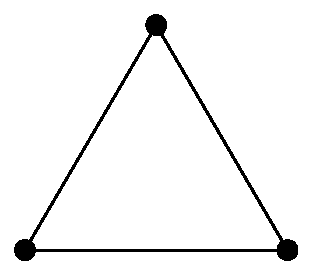
\includegraphics[totalheight=.8in]{intrograph}
\end{picture}
\begin{picture}(0,0)
  \put(-157,0){$t-1$ color choices}
  \put(-22,50){$t$ color choices}
  \put(5,0){$t-2$ color choices}
\end{picture}
\end{center}
\caption{Proper $t$-colorings of $K_3$.}\label{intrographfig}
\end{figure}

The overlaying of figures reminds me of two of my other favorite \LaTeX \ commands: {\tt $\backslash$vspace} and {\tt $\backslash$hspace}. For example, they allow you to place
just about

\vspace{.5in}
\hspace{2in}
anything

\vspace{-.5in}
\hspace{5in}
anywhere.

\vspace{.5in}
\noindent
This can be very useful, e.g., for presentations in which you might move pictures around.

%%%%%%%%%%%%%%%%%%%%%%%%%%%%%%%%%%%%%%%%%%%%%%%%%%%%%%%%%%%%%%%%%%%%%%%%%%%

\section{Bibliographic Stuff}

For references like \cite[Section 2]{athanasiadismagic} I recommend using {\tt bibtex}; it means that you have to do only minimal work, especially when you get the entries
from \emph{MathSciNet}. I keep all the references I've ever used in the same file and use this in all my documents\dots

If you could use an index at the end of your document, use {\tt makeindex}---one of best reasons to use \LaTeX \ if you're writing a book.




%\chapter*{Appendix A: Triangulations of Polytopes}
%\addcontentsline{toc}{chapter}{Appendix A: Triangulations of Polytopes}

\appendix{Appendix A: Triangulations of Polytopes}

This creates an appendix, which is not numbered (and therefore has to be added to the table of contents semi-manually).

For code, the {\tt verbatim} environment (maybe in conjunction with $\backslash${\tt include}) is helpful:

\begin{verbatim}
It reproduces text
  exactly
    as
      it
        is
typed.
\end{verbatim}

Good luck and enjoy writing!
\end{document}






% TLC




%==============%
% Bibliography %
%==============%

% BibTex %
%\bibliographystyle{amsplain}
%\addcontentsline{toc}{chapter}{Bibliography}
%\singlespacing
%\bibliography{thesis}

%BibLatex :
\printbibliography

\end{document}




% TLC May 2019